%%%%%%%%%%%%%%%%%%%%%%%%%%%%%%%%%%%%%%%%%%%%%%%%%%%%%%%%%%%%%%%%%%%%%%%%%%%%%%%%
% Author : Adam Pribyl, Tomas Polasek (template)
% Description : Seventh exercise in the Introduction to Game Development course.
%   It deals with the creation of a Game Design Document, presenting a short 
%   pitch for a potential game project.
%%%%%%%%%%%%%%%%%%%%%%%%%%%%%%%%%%%%%%%%%%%%%%%%%%%%%%%%%%%%%%%%%%%%%%%%%%%%%%%%

\documentclass[a4paper,10pt,english]{article}

\usepackage[left=2.50cm,right=2.50cm,top=1.50cm,bottom=2.50cm]{geometry}
\usepackage[utf8]{inputenc}

% Hyper-Text References
\usepackage{hyperref}
\hypersetup{colorlinks=true, urlcolor=grey}

% Drawing Images and Graphs
\usepackage{tikz}
\usepackage{pgfplots}

% Page Utilities
\usepackage{graphicx}

% Image Sub-Captions
\usepackage{subcaption}

\newcommand{\ph}[1]{\textit{[#1]}}


\title{%
GNOMER Pitch Document%
}
\author{%
Adam Přibyl (xpribya00)%
}
\date{}

\begin{document}

\maketitle
\thispagestyle{empty}

\begin{figure}[h!]
    \centering
    
\includegraphics[width=0.7\textwidth]{title.png}
    \label{fig:title}
\end{figure}

{%
\large

\begin{itemize}

\item[] \textbf{Title:} \ph{GNOMER}

\item[] \textbf{Genre:} \ph{Deckbuilder Roguelike}

\item[] \textbf{Style:} \ph{2D, Pixelart, Topdown}

\item[] \textbf{Platform:} \ph{Windows, OSX, Linux}

\item[] \textbf{Market:} \ph{Roguelike players / Experienced deckbuilder enjoyers}

\item[] \textbf{Elevator Pitch:} \ph{Open card booster packs and use combinations of opened effect cards to defeat hordes of gnomes}

\end{itemize}
}

\section*{\centering ''A game that simply scratches the right part of the brain''}

Everyone has at least heard of a trading card game. Nothing compares to the feeling of opening something precious from a deck of cards when we were kids (some of us as grown-ups). That's exactly the feeling that playing Gnomer brings. The player opens up decks of cards and uses them to fight hordes of gnomes that, with the right combination of cards, basically crumble under your fingers. So in all respects the game simply scratches the right part of the brain and is very satisfying. 

\subsection*{Introduction}
Gnomer is a game in which the player collects effect cards and forms their combinations, using them to fight against hordes of gnomes. These cards range from one-hit upgrades to cards that completely turn the gameplay 180 degrees (such as cards that change the behavior of weapons or even the enemies themselves).

\subsection*{Background}
Gnomer takes its main inspiration from TGC games like Pokémon and Magic: The Gathering. The popularity of building a deck of cards with special effects working together in video games is confirmed by the recent success of Balatro.
Another game that Gnomer is inspired by is Vampire Survivors, here we can find similarities in the destruction of hordes, which in Vampire Survivors is considered almost a drug (because it is so satisfying). So again, it adds to the overall satisfaction

\subsection*{Setting}
Gnomer has no story as such, but it has a distinctive setting: the game takes place in a classic medieval world containing magic. In this world live many different creatures, and one of them are the Gnomes, who are simply seen as pests in this world that need to be exterminated (or degnomed ?). So the player takes control of one degnomer (which is a job like any other in this world) and sets out to mow down the gnome hordes.

\subsection*{Features}
In the background section we have already explained what the main driving currents are for each feature and why they are proven in the industry but still not so common in this combination. Now we will go through them one by one in detail

\subsubsection*{ - Effect cards}
\begin{center}
    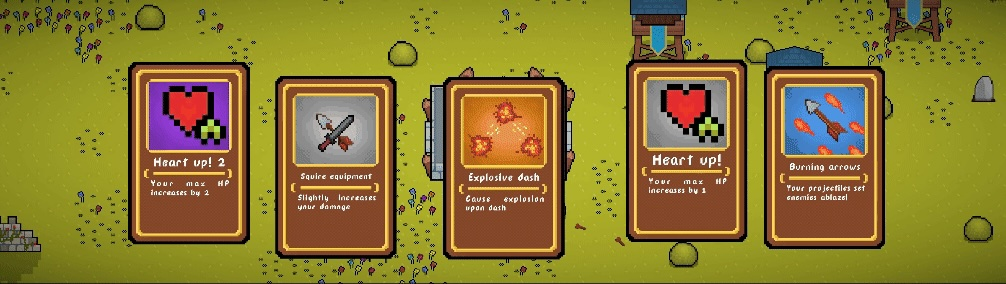
\includegraphics[width=1\textwidth]{cards.jpg}
\end{center}
The main mechanic of Gnomer is the use of effect cards, which are divided into passive and active cards:\newline

\textbf{Passive cards}\newline
These are cards that are always activated, for example cards that improve a certain stat: such as increasing the number of lives or damage the player does. Such a card is also for example a card that will ignite the player's arrows, these will ignite the enemies, here comes the catch such a card can be used together with another card that will say that the enemies that die because of the fire will explode after their death and will grant damage to other enemies around them. In this way the player composes combinations of cards that work together.

\textbf{Active cards}\newline
These are cards that the player must activate, they wait in his inventory before he activates them, some are disposable and others he can use again after a certain amount of time. Another such card is for example the fireball, which the player can send to his enemies, another such card is for example the building cards, which after activation the player can place anywhere on the map and this building will then help him: for example shoot gnomes or the player will generate lives.


\subsubsection*{ - Booster Packs}
\begin{center}
    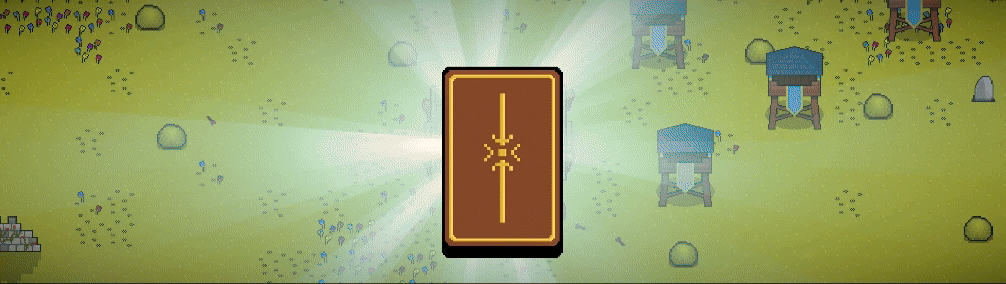
\includegraphics[width=1\textwidth]{boosterPack.jpg}
\end{center}

The game capitalizes on the popularity of opening lootboxes, which has become an integral part of any popular multiplayer game over the past few years. Players love opening packages with unknown content, chance and luck simply makes them exciting. It is essentially a form of gambling that has guided mankind for centuries and is more popular than ever. Of course, the player is not risking his money here, but only the in-game currency, making it a very fun and harmless form. This mechanic sets the game apart from other roguelike games, and with countless possible card combinations waiting for you for every run, the game bites and doesn't let go.

\subsection*{Genre}
The main genre of the game is a Roguelike, which means that after each death the player starts from the beginning, what sets roguelike and roguelite apart is that in roguelike game you can gain permanent upgrades that will help you on your next run. \newline
The second genre is Deckbuilder, which means that the player builds a deck of cards and decides which cards work better with his current deck.
The game is a mix of several tried and working genres and mechanics, so it has a very solid foundation and differs from others in each genre just by fusing with other genres and mechanics

\subsection*{Platform}
At the moment the launch is planned for Windows, OSX and Linux. Since the control scheme works very well on the controller, it is certainly possible to add support for game consoles after eventual success on these platforms.

\subsection*{Style}
The visual style is very simple, it is a 2D pixelart game. Working with pixels allows us to create very fast graphics for the game. The visual style is very colourful and varied, the characters move with an almost comical swaying gait and it works beautifully with the light-hearted atmosphere of the game. The simple sprites are complemented by complex visual effects of glows and similar magical elements, which beautifully accentuates the magic.

\begin{figure}[h]

\centering

\begin{subfigure}{0.29\linewidth}
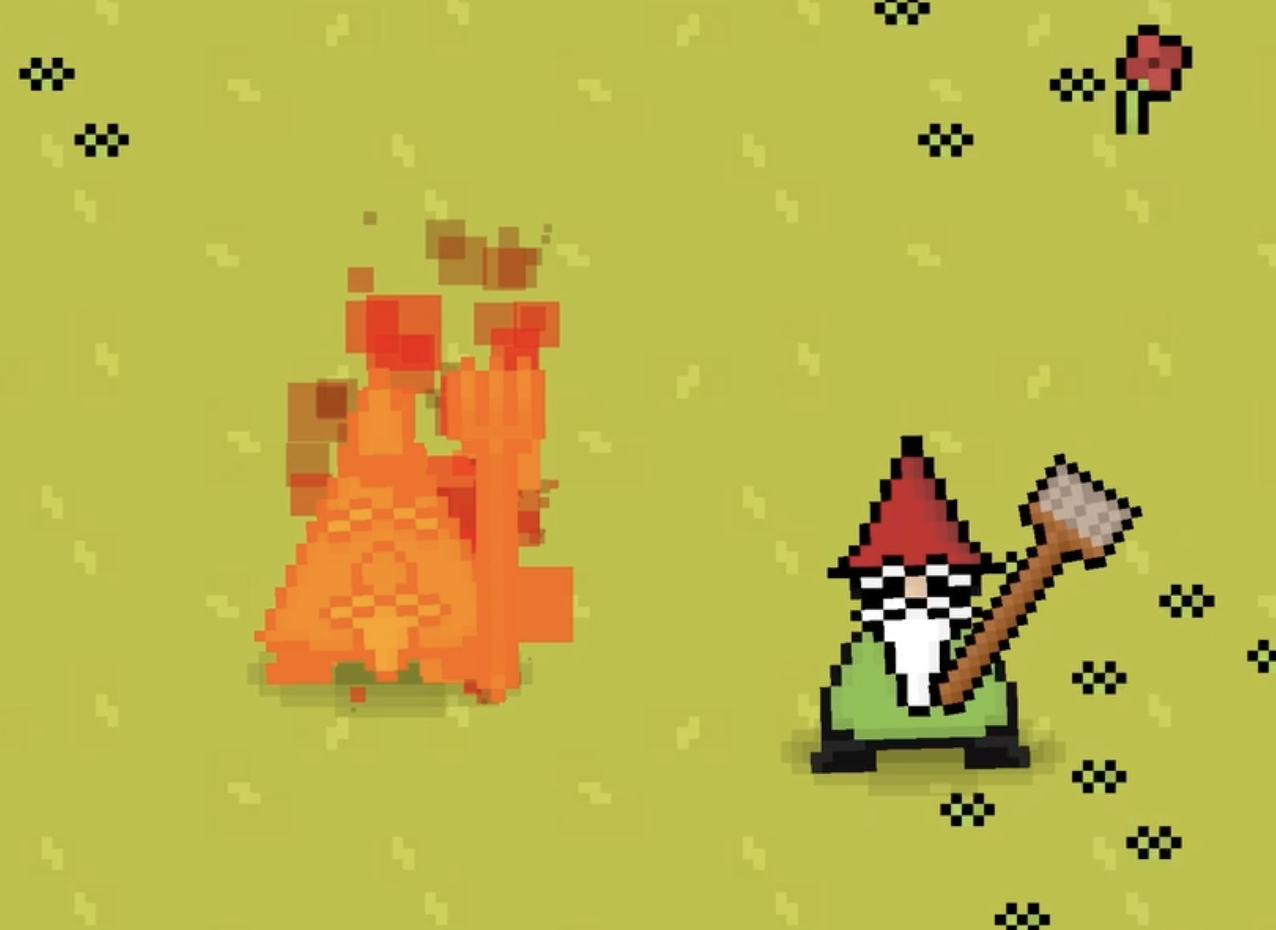
\includegraphics[width=\linewidth]{gnomes.png}
\captionof{figure}{Gnomes}
\label{Fig:Style1A}
\end{subfigure}\hfill
%
\begin{subfigure}{0.29\linewidth}
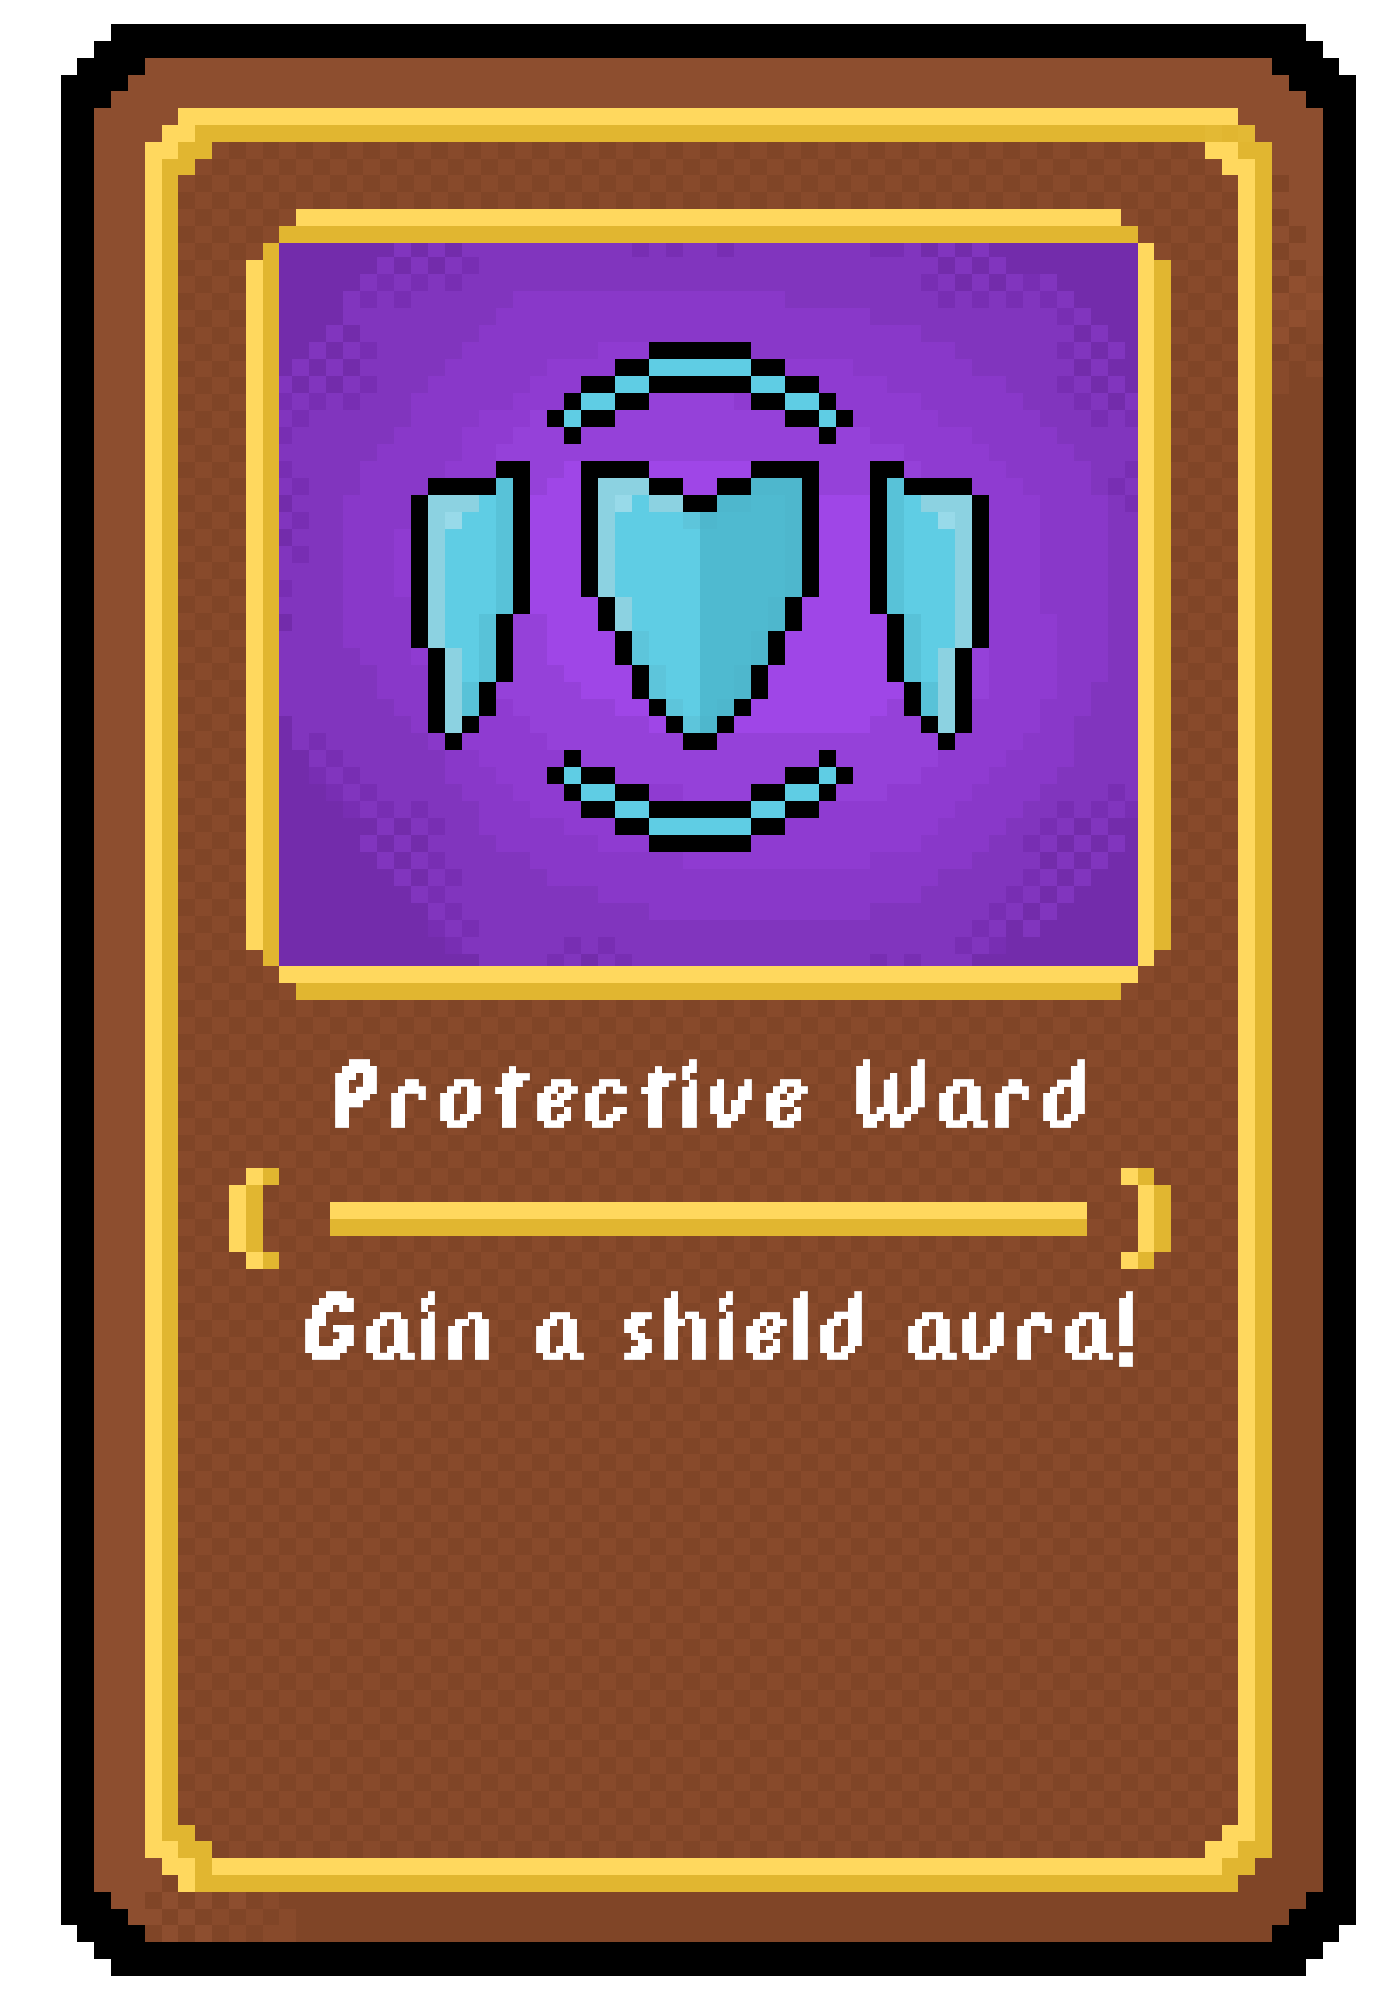
\includegraphics[width=\linewidth]{card.png}
\captionof{figure}{Effect card}
\label{Fig:Style1B}
\end{subfigure}\hfill
%
\begin{subfigure}{0.29\linewidth}

\includegraphics[width=\linewidth]{pack.png}
\captionof{figure}{Booster pack}
\label{Fig:Style1C}
\end{subfigure}

\end{figure}

\subsection*{Links}
\begin{itemize}
    \item[] \textbf{Steam page} \href{https://store.steampowered.com/app/3112030/Gnomer/}{https://store.steampowered.com/app/3112030/Gnomer/}
    \item[] \textbf{Team Ruby website} \href{https://teamrubygames.com/}{https://teamrubygames.com/}
    \item[] \textbf{Vortex article} \href{https://www.vortex.cz/vyzkousejte-si-demo-ceskeho-roguelike-gnomer/}{https://www.vortex.cz/vyzkousejte-si-demo-ceskeho-roguelike-gnomer/}
    \item[] \textbf{Interview about the game} \href{https://youtu.be/oJjDMNefwME?t=3581}{https://youtu.be/oJjDMNefwME?t=3581}
    
\end{itemize}


\begin{center}
    
\includegraphics[width=0.15\textwidth]{RubyLogo.png}
\end{center}

\end{document}
